\chapter{Method/Approach (theoretical)}
Extracting information from documents written in text is not a simple task due to the nature of the complexity of natural language. \cite{t2m_1} identified several obstacles to performing the information extraction: \textit{Syntactic Leeway} describes the problem of inconsistency between the semantic and syntactic aspects of the textual representation. \textit{Atomicity} refers to the problem of adequately mapping the phase-activities. \textit{Relevance} checks whether some part of the text input is irrelevant to the process model, such as examples offered by authors, which helps the human reader to understand the described process but introduces noise for information extraction. \textit{Referencing} deals with the question of how to identify the references between sentences, e.g., the pronouns "This" and "it", from the sentence "After this step, it will be delivered to ...".

\begin{figure}[h]
    \centering
    \caption{Overview of pre-processing}
    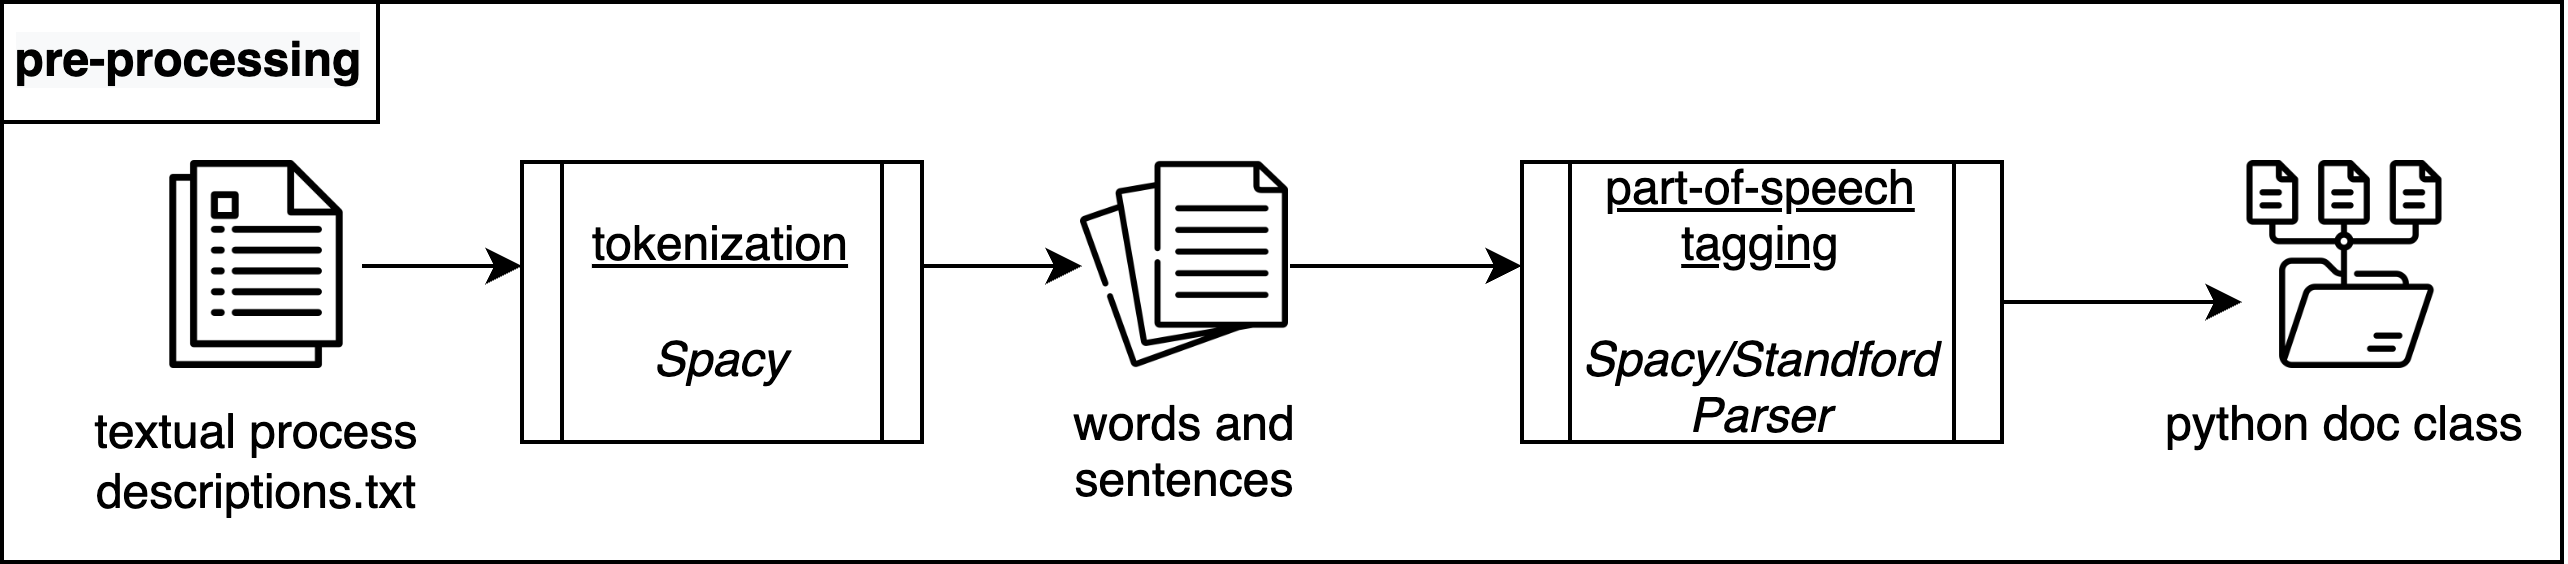
\includegraphics[width=0.8\textwidth]{tum-resources/images/theoretical_extraction_pre.png}
\end{figure}

Our approach will consider using textual process descriptions as input files in the format of \textit{.txt}. In the first step, the input file will be pre-processed. The documents will be split into sentences and words using tokenization. Correctly identifying the end of sentences is crucial for further information processing. Then, the words in the sentence should be tagged with a proper grammatical label using the part-of-speech technique so that the relationship between words can be analyzed. An essential step of this part is to identify the business activities. \cite{t2m_5} and \cite{complement_1} suggest that the identification can be achieved by the pre-defined rules based on the grammatical properties of the words. Once the business activities are identified, they can be used as the fundament of the work.


This step should also tackle the problem of active and passive voice. After all tasks in pre-processing, the tagged documents will be used for the analysis of the relationship between sentences.

\begin{figure}[h]
    \centering
    \caption{Overview of processing}
    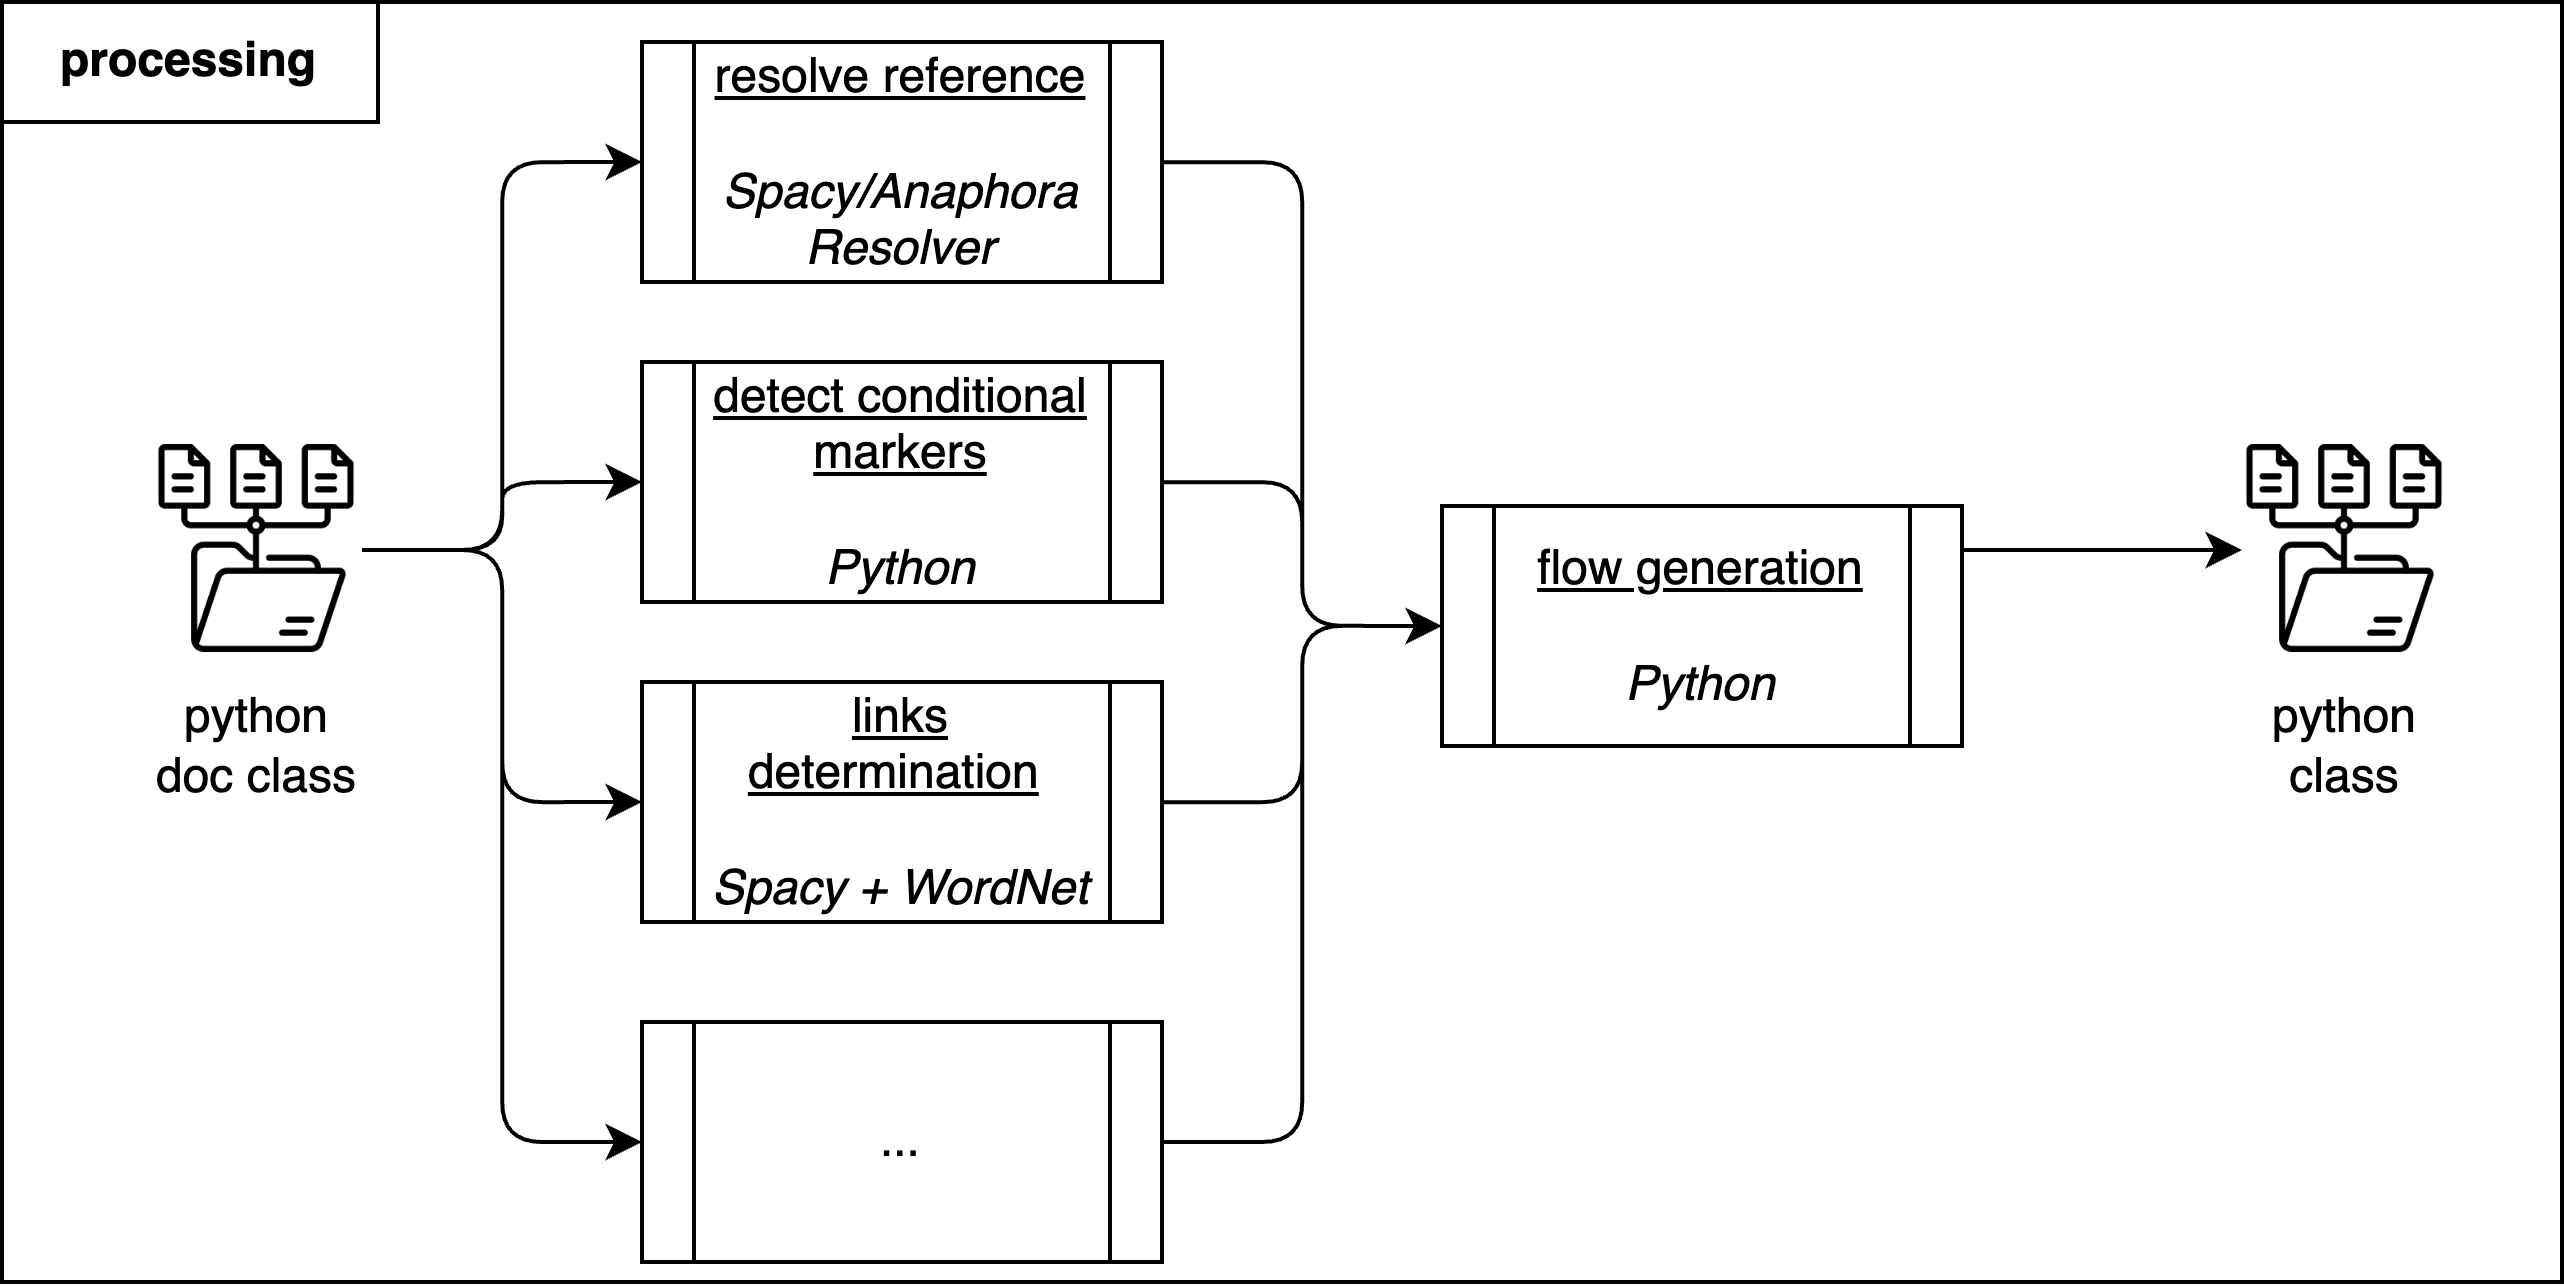
\includegraphics[width=0.8\textwidth]{tum-resources/images/theoretical_extraction_pro.png}
\end{figure}

The primary step of information extraction is text-level analysis, where sentences' sequential, conditional relationships will be exploited. In the pre-processing, the work has already tackled the problem of business activity identification. However, the identified business activities might not be complete because of the referencing problem and active/passive voice problem. In the central part of the work, the anaphora resolution problem has to be solved, which refers to the word that represents a word or a phrase that occurred beforehand \cite{literature_review_4}. Next, the approach has to solve the problem of finding conditional relationships between sentences. The conditional relationship is usually represented through a conditional word like "if", "else", "otherwise", etc. Finding these relationships is very crucial for the construction of logical conjunctions in the business model. Another essential task in text-level analysis is flow generation. A flow indicates how the business activities are related to each other and could be used to translate the processed information above into the business process model \cite{t2m_1}.


After the flows of the model are generated, the post-processing phase could now be performed. Post-processing is about generating BPMN representation using the information acquired in the last two steps. \cite{t2m_1} suggests four steps of model generation: nodes creation, sequence flows construction, dummy elements removal, and open ends finishing. The nodes and edges will be created first to create the BPMN model. Then the dummy actions will be skipped, which are used to insert between gateways. Finally, the Start and the End events are to be created. As a result, all necessary elements of the BPMN model is created. 

%\cite{complement_1} illustrate us to additionally implement a web interface that eases to use of the text document to BPMN model transmission service. The web interface should take the text description as input and then will represent the BPMN model in the webpage after the text is processed with our model in the backend.

\begin{figure}[h]
    \centering
    \caption{Overview of post-processing}
    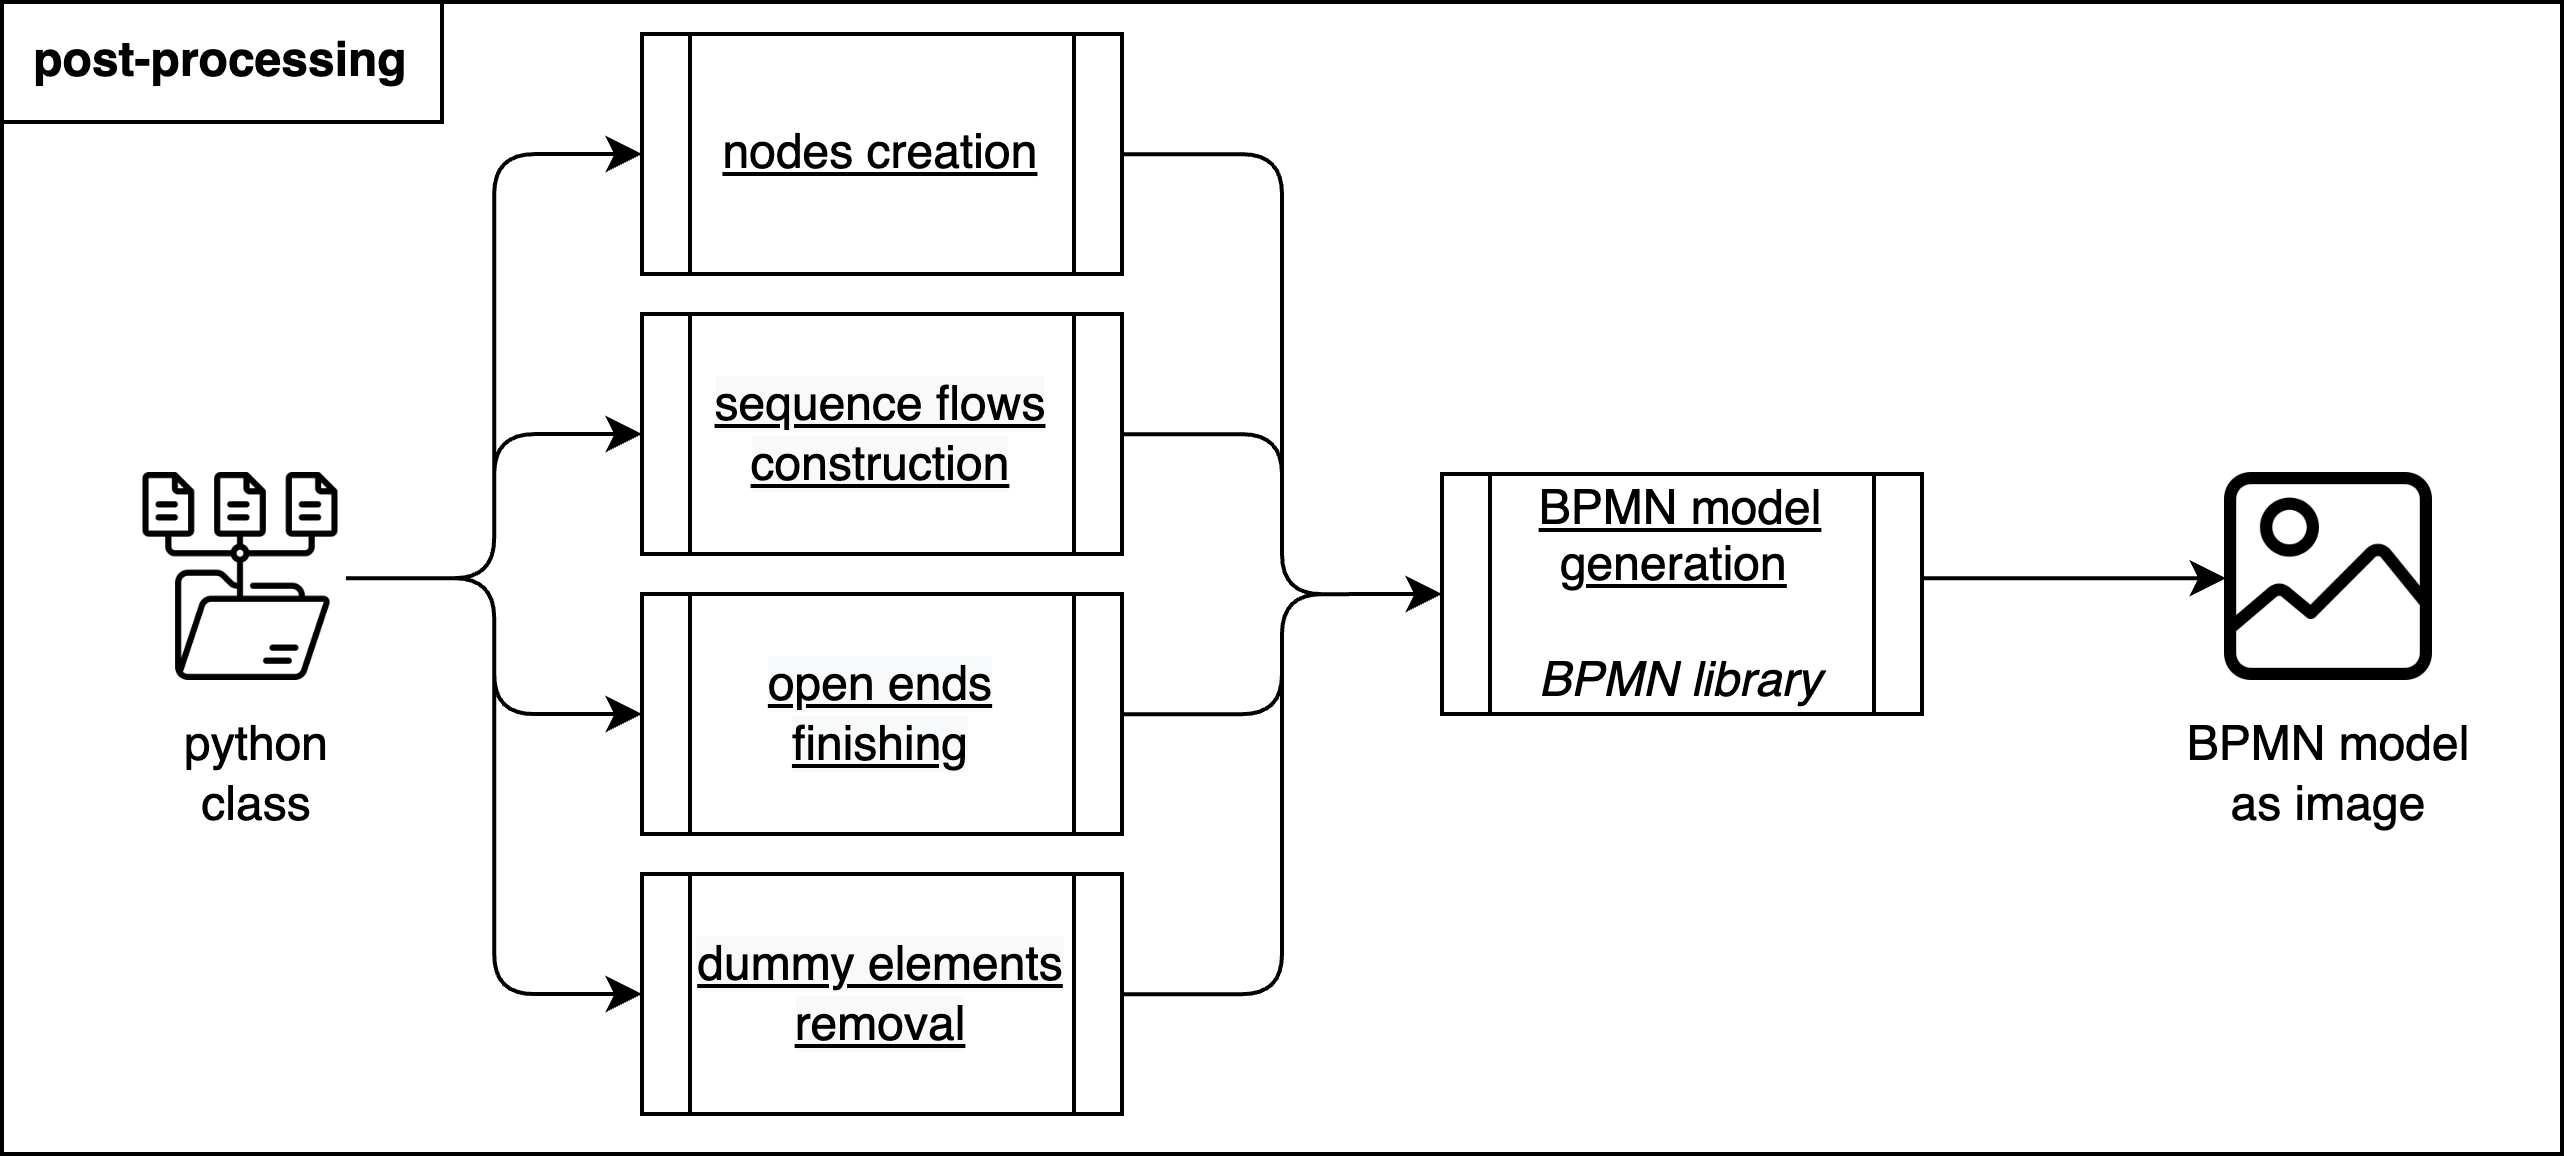
\includegraphics[width=0.8\textwidth]{tum-resources/images/theoretical_extraction_post.png}
\end{figure}
